% ===========================================================================
% Diapositivas Beamer - Trabajo Final, Asignatura Inteligencia Artificial
% Titulo: Prediccion de Riesgo Financiero en PYMES Colombianas mediante
%         Machine Learning con Datos del SIREM (2016-2024)
% Autores: Juan Camilo Perea, German
% Universidad de Ibague - 2026
% ===========================================================================

\documentclass[10pt, aspectratio=169, xcolor=dvipsnames]{beamer}

% --- Idioma y codificacion ---
\usepackage[spanish, es-tabla]{babel}
\usepackage[utf8]{inputenc}
\usepackage[T1]{fontenc}
\usepackage{lmodern}

% --- Matematicas (para \checkmark) ---
\usepackage{amssymb}

% --- Tablas y figuras ---
\usepackage{booktabs}
\usepackage{array}
\usepackage{graphicx}

% --- Tipografia y miscelaneos ---
\usepackage{microtype}

% --- Tema Beamer + colores Universidad de Ibague (azul institucional) ---
\usetheme{Madrid}
\usecolortheme{seahorse}

\definecolor{uibblue}{RGB}{0,70,127}
\definecolor{uibblue80}{RGB}{51,108,154}
\definecolor{uibgold}{RGB}{200,160,30}

\setbeamercolor{structure}{fg=uibblue}
\setbeamercolor{palette primary}{bg=uibblue, fg=white}
\setbeamercolor{palette secondary}{bg=uibblue80, fg=white}
\setbeamercolor{palette tertiary}{bg=uibblue, fg=white}
\setbeamercolor{title}{fg=white}
\setbeamercolor{frametitle}{bg=uibblue, fg=white}
\setbeamercolor{block title}{bg=uibblue80, fg=white}
\setbeamercolor{block body}{bg=uibblue!5, fg=black}
\setbeamercolor{itemize item}{fg=uibblue}
\setbeamercolor{itemize subitem}{fg=uibblue80}
\setbeamercolor{section in head/foot}{bg=uibblue, fg=white}
\setbeamercolor{author in head/foot}{bg=uibblue, fg=white}
\setbeamercolor{title in head/foot}{bg=uibblue80, fg=white}
\setbeamercolor{date in head/foot}{bg=uibblue, fg=white}

\setbeamerfont{frametitle}{series=\bfseries}
\setbeamertemplate{navigation symbols}{}

% --- Comandos auxiliares ---
\newcommand{\zaltscore}{Z\textquotesingle\textquotesingle-Score}

% --- Ruta de figuras ---
\graphicspath{{../../reports/figures/}}

% --- Metadatos ---
\title[ML para riesgo financiero en PYMES]{Predicci\'on de Riesgo Financiero en PYMES Colombianas\\ mediante Machine Learning con Datos del SIREM (2016--2024)}
\subtitle{Trabajo final --- Asignatura Inteligencia Artificial}
\author[Perea \& German]{Juan Camilo Perea \and German}
\institute[U. Ibagu\'e]{Universidad de Ibagu\'e --- Facultad de Ingenier\'ia}
\date{2026}

\begin{document}

% =====================================================================
% Slide 1 - Titulo
% =====================================================================
{\setbeamercolor{background canvas}{bg=uibblue}
\setbeamercolor{normal text}{fg=white}
\begin{frame}[plain]
\vspace{0.6cm}
\centering
{\color{white}\Large\bfseries Universidad de Ibagu\'e\par}
{\color{white}\large Facultad de Ingenier\'ia --- Inteligencia Artificial\par}
\vspace{1.0cm}
{\color{white}\Large\bfseries Predicci\'on de Riesgo Financiero en\par PYMES Colombianas mediante \emph{Machine Learning}\par}
{\color{white}\large con Datos del SIREM (2016--2024)\par}
\vspace{1.0cm}
{\color{white}\normalsize Juan Camilo Perea \quad\textbar\quad German\par}
\vspace{0.6cm}
{\color{white!85!uibblue}\small Trabajo final --- 2026\par}
\end{frame}}

% =====================================================================
% Slide 2 - Agenda
% =====================================================================
\begin{frame}{Agenda}
\begin{enumerate}
  \item Contexto y brecha en la literatura
  \item Estado del arte y objetivos
  \item Metodolog\'ia y datos
  \item Resultados sobre test nacional
  \item Validaci\'on en Ibagu\'e
  \item Discusi\'on, robustez y conclusiones
\end{enumerate}
\end{frame}

% =====================================================================
% Slide 3 - Contexto y brecha
% =====================================================================
\begin{frame}{Contexto y brecha}
\begin{itemize}
  \item PYMES $>$ 90\% del tejido empresarial formal de Colombia.
  \item Alta mortalidad temprana y acceso limitado a financiaci\'on [Higuera 2021].
  \item Modelos cl\'asicos (Altman, Ohlson) se degradan fuera de su contexto [Grice 2003; Bouwmeester 2020].
  \item Solo 19 estudios PYME$+$ML en una d\'ecada, casi ninguno en LATAM [Abubakar 2025].
  \item El SIREM publica estados financieros NIIF de 38\,245 PYMES: fuente p\'ublica desaprovechada.
\end{itemize}
\end{frame}

% =====================================================================
% Slide 4 - Estado del arte: 7 ejes
% =====================================================================
\begin{frame}{Estado del arte: s\'intesis condensada}
\small
\begin{tabular}{@{}p{3.2cm} p{8.6cm}@{}}
\toprule
\textbf{Eje} & \textbf{Hallazgo y referencias clave} \\
\midrule
Riesgo PYME           & Vulnerabilidad financiera persistente [Cultrera 2016; Senaya 2025]. \\
M\'etodos cl\'asicos  & Z-Score y Ohlson degradan fuera de contexto [Grice 2003; Qiu 2020]. \\
ML para riesgo        & XGBoost domina la SLR de 207 estudios [Dasilas 2024; Boumhidi 2025]. \\
Sistemas web          & Un solo prototipo LATAM identificado [Mayorga-Lira 2023]. \\
NIIF Colombia         & Decreto 2015 alinea SIREM con NIIF [DAFP 2015]. \\
Interpretabilidad     & TreeSHAP estable y eficiente [Lundberg 2020; Lin 2024]. \\
Validaci\'on temporal & Split cronol\'ogico estricto necesario [Bortolotti 2024]. \\
\bottomrule
\end{tabular}
\end{frame}

% =====================================================================
% Slide 5 - Objetivos
% =====================================================================
\begin{frame}{Objetivos}
\textbf{General.} Dise\~nar e implementar un modelo de \emph{Machine Learning} supervisado que clasifique el riesgo financiero (bajo/medio/alto) de PYMES colombianas y validarlo en Ibagu\'e.

\medskip
\textbf{Espec\'ificos.}
\begin{enumerate}
  \item Calcular 18 indicadores financieros sobre el universo SIREM 2016--2024.
  \item Construir una etiqueta triangulada (\zaltscore{} + heur\'istica + cuartiles).
  \item Comparar tres modelos: regresi\'on log\'istica, Random Forest y XGBoost.
  \item Evaluar con F1-macro y AUC-PR bajo validaci\'on temporal estricta.
  \item Interpretar v\'ia TreeSHAP global y local.
  \item Validar el modelo nacional sobre el holdout de Ibagu\'e.
\end{enumerate}
\end{frame}

% =====================================================================
% Slide 6 - Pipeline metodologico
% =====================================================================
\begin{frame}{Pipeline metodol\'ogico (8 fases)}
\centering
\small
\setlength{\tabcolsep}{4pt}
\renewcommand{\arraystretch}{1.15}
\begin{tabular}{@{}c@{ $\to$ }c@{ $\to$ }c@{ $\to$ }c@{}}
\toprule
\textbf{F1} & \textbf{F2} & \textbf{F3} & \textbf{F4} \\
Indicadores + EDA & Etiquetado triangulado & Feature engineering & Split temporal + holdout \\
\bottomrule
\end{tabular}
\vspace{0.3cm}
\begin{tabular}{@{}c@{ $\to$ }c@{ $\to$ }c@{ $\to$ }c@{}}
\toprule
\textbf{F5} & \textbf{F6} & \textbf{F7} & \textbf{F8} \\
Modelado (4 modelos) & Evaluaci\'on + SHAP & Validaci\'on Ibagu\'e & Discusi\'on comparativa \\
\bottomrule
\end{tabular}
\medskip
\begin{itemize}
  \item Reproducibilidad: \texttt{random\_state=42}, notebooks 03--10, c\'odigo en \texttt{src/}.
  \item Carga via \texttt{cargar\_consolidado()} (normaliza 105 columnas con \emph{mojibake}).
\end{itemize}
\end{frame}

% =====================================================================
% Slide 7 - Datos: SIREM + Ibague
% =====================================================================
\begin{frame}{Datos: SIREM y caso Ibagu\'e}
\begin{itemize}
  \item 4 datasets SIREM ($\sim$9,17 GB): Car\'atula, Situaci\'on Financiera, Resultados, Flujo de Efectivo.
  \item ETL pivoteado: \textbf{203\,104 obs}\,$\times$\,230 columnas, \textbf{38\,245 PYMES} NIIF Pymes Grupo 2.
  \item Cobertura temporal: 2016--2024 (panel desbalanceado).
  \item Cruce con C\'amara de Comercio Ibagu\'e: \textbf{61 NITs} ($\to$ 359 obs.\ holdout).
  \item Limpieza NIT: SIREM almacena \texttt{"900,152,104"}; CCI usa 10 d\'igitos, SIREM 9 d\'igitos.
  \item Sesgo de selecci\'on: solo PYMES con capacidad de reporte NIIF formal.
\end{itemize}
\end{frame}

% =====================================================================
% Slide 8 - Etiquetado triangulado
% =====================================================================
\begin{frame}{Etiquetado triangulado (Fase 2)}
\begin{itemize}
  \item \textbf{A}: zonas Altman umbrales originales (1{,}1 / 2{,}6) --- descartado, $\kappa_{A,B}=0{,}234$.
  \item \textbf{B}: terciles emp\'iricos del \zaltscore{} sobre el dataset.
  \item \textbf{C}: heur\'istica de 5+5 se\~nales con \emph{terciles por indicador} (no umbrales fijos).
  \item Recalibrar C con terciles emp\'iricos elev\'a $\kappa_{B,C}$ de 0{,}304 a \textbf{0{,}446} ($\geq 0{,}4$ $\checkmark$).
  \item \textbf{Etiqueta final} = consenso B$\equiv$C; \emph{riesgo medio} cuando hay discrepancia.
  \item Distribuci\'on resultante: \textbf{16,8\% bajo / 66,4\% medio / 16,8\% alto}.
\end{itemize}
\end{frame}

% =====================================================================
% Slide 9 - Feature engineering
% =====================================================================
\begin{frame}{Ingenier\'ia de caracter\'isticas (71 \emph{features})}
\centering
\small
\setlength{\tabcolsep}{6pt}
\renewcommand{\arraystretch}{1.1}
\begin{tabular}{@{}l c l@{}}
\toprule
\textbf{Familia} & \textbf{N} & \textbf{Ejemplos} \\
\midrule
Indicadores base + \zaltscore{}              & 19 & \texttt{razon\_corriente, roa, z\_score\_altman} \\
Variaciones interanuales (\texttt{\_d1})     & 18 & \texttt{margen\_neto\_d1, razon\_deuda\_d1} \\
Crecimientos multi-a\~no (\texttt{\_g2/\_g3})& 6  & \texttt{roa\_g3, razon\_deuda\_g2} \\
Escala / estructura                          & 4  & \texttt{log\_activos, ac/at, pc/pt} \\
Temporales                                   & 2  & \texttt{anyo\_num, dummy\_covid\_2020} \\
\emph{Dummies} categ\'oricas                 & 22 & CIIU 12 + sociedad 4 + departamento 6 \\
\midrule
\textbf{Total}                               & \textbf{71} & winsorizado p1--p99 (51 columnas continuas) \\
\bottomrule
\end{tabular}
\medskip
\begin{itemize}
  \item Cero columnas 100\% nulas; cero duplicados (NIT, A\~NO); \emph{dummies} suman 1 por grupo.
\end{itemize}
\end{frame}

% =====================================================================
% Slide 10 - Particion temporal y no-leakage
% =====================================================================
\begin{frame}{Partici\'on temporal y holdout Ibagu\'e}
\begin{itemize}
  \item \textbf{Train} 2016--2021 --- 108\,522 obs.
  \item \textbf{Validation} 2022 --- 26\,878 obs.
  \item \textbf{Test} 2023--2024 --- 50\,957 obs.
  \item \textbf{Holdout Ibagu\'e} --- 359 obs (61 PYMES).
  \item Cuatro \emph{asserts} de no-fuga: ning\'un NIT Ibagu\'e en splits nacionales.
  \item Exclusi\'on \textbf{ANIO=2017} del nacional: 99,1\% Z-Score nulos (anomal\'ia SIREM).
  \item Delta m\'aximo entre splits: 4,5 pp ($\leq 5$ pp $\checkmark$).
\end{itemize}
\end{frame}

% =====================================================================
% Slide 11 - Modelado
% =====================================================================
\begin{frame}{Modelado: cuatro candidatos}
\centering
\small
\setlength{\tabcolsep}{6pt}
\renewcommand{\arraystretch}{1.1}
\begin{tabular}{@{}l l c c@{}}
\toprule
\textbf{Modelo} & \textbf{Hiperpar\'ametros ganadores} & \textbf{F1-macro val} & \textbf{Fits} \\
\midrule
Regresi\'on log\'istica & \texttt{C=10}, \texttt{cw=balanced}                                  & 0,7993 & 4 \\
Random Forest          & \texttt{n=500}, \texttt{depth=None}, \texttt{mss=10}                  & 0,9948 & 18 \\
XGBoost (sw)           & \texttt{depth=8}, \texttt{lr=0,1}, \texttt{ss=0,8}, \texttt{cs=1,0}   & \textbf{0,9979} & 24 \\
XGBoost + SMOTE        & \texttt{depth=4}, \texttt{lr=0,05}                                   & 0,9957 & 24 \\
\bottomrule
\end{tabular}
\medskip
\begin{itemize}
  \item 70 \emph{fits} totales --- GPU NVIDIA RTX 2060, \texttt{device='cuda'} (4$\times$ \emph{speedup}).
  \item \texttt{early\_stopping\_rounds=30} sustituye \texttt{n\_estimators} (best\_iteration=221).
\end{itemize}
\end{frame}

% =====================================================================
% Slide 12 - Resultados test nacional
% =====================================================================
\begin{frame}{Resultados sobre test nacional ($n=50\,957$)}
\centering
\small
\setlength{\tabcolsep}{6pt}
\renewcommand{\arraystretch}{1.15}
\begin{tabular}{@{}l c c c c@{}}
\toprule
\textbf{Modelo} & \textbf{Acc} & \textbf{F1-macro} & \textbf{AUC-ROC OvR} & \textbf{AUC-PR macro} \\
\midrule
\textbf{XGBoost (sw)} & \textbf{0,9975} & \textbf{0,9972} & \textbf{1,0000} & \textbf{1,0000} \\
XGBoost + SMOTE      & 0,9962 & 0,9956 & 1,0000 & 0,9999 \\
Random Forest        & 0,9950 & 0,9943 & 0,9999 & 0,9998 \\
Regresi\'on log.\    & 0,8210 & 0,8105 & 0,9533 & 0,8932 \\
\bottomrule
\end{tabular}
\medskip
\begin{itemize}
  \item Sin \emph{drift} train$\to$val$\to$test: $1{,}0000 \to 0{,}9979 \to 0{,}9972$ (gap $-0{,}07$ pp).
  \item Ventaja XGBoost vs.\ \emph{baseline} log\'istico: $+18{,}67$ pp en test ($\geq 5$ pp $\checkmark$).
\end{itemize}
\end{frame}

% =====================================================================
% Slide 13 - Matriz de confusion + ROC/PR
% =====================================================================
\begin{frame}{Matriz de confusi\'on y separabilidad}
\centering
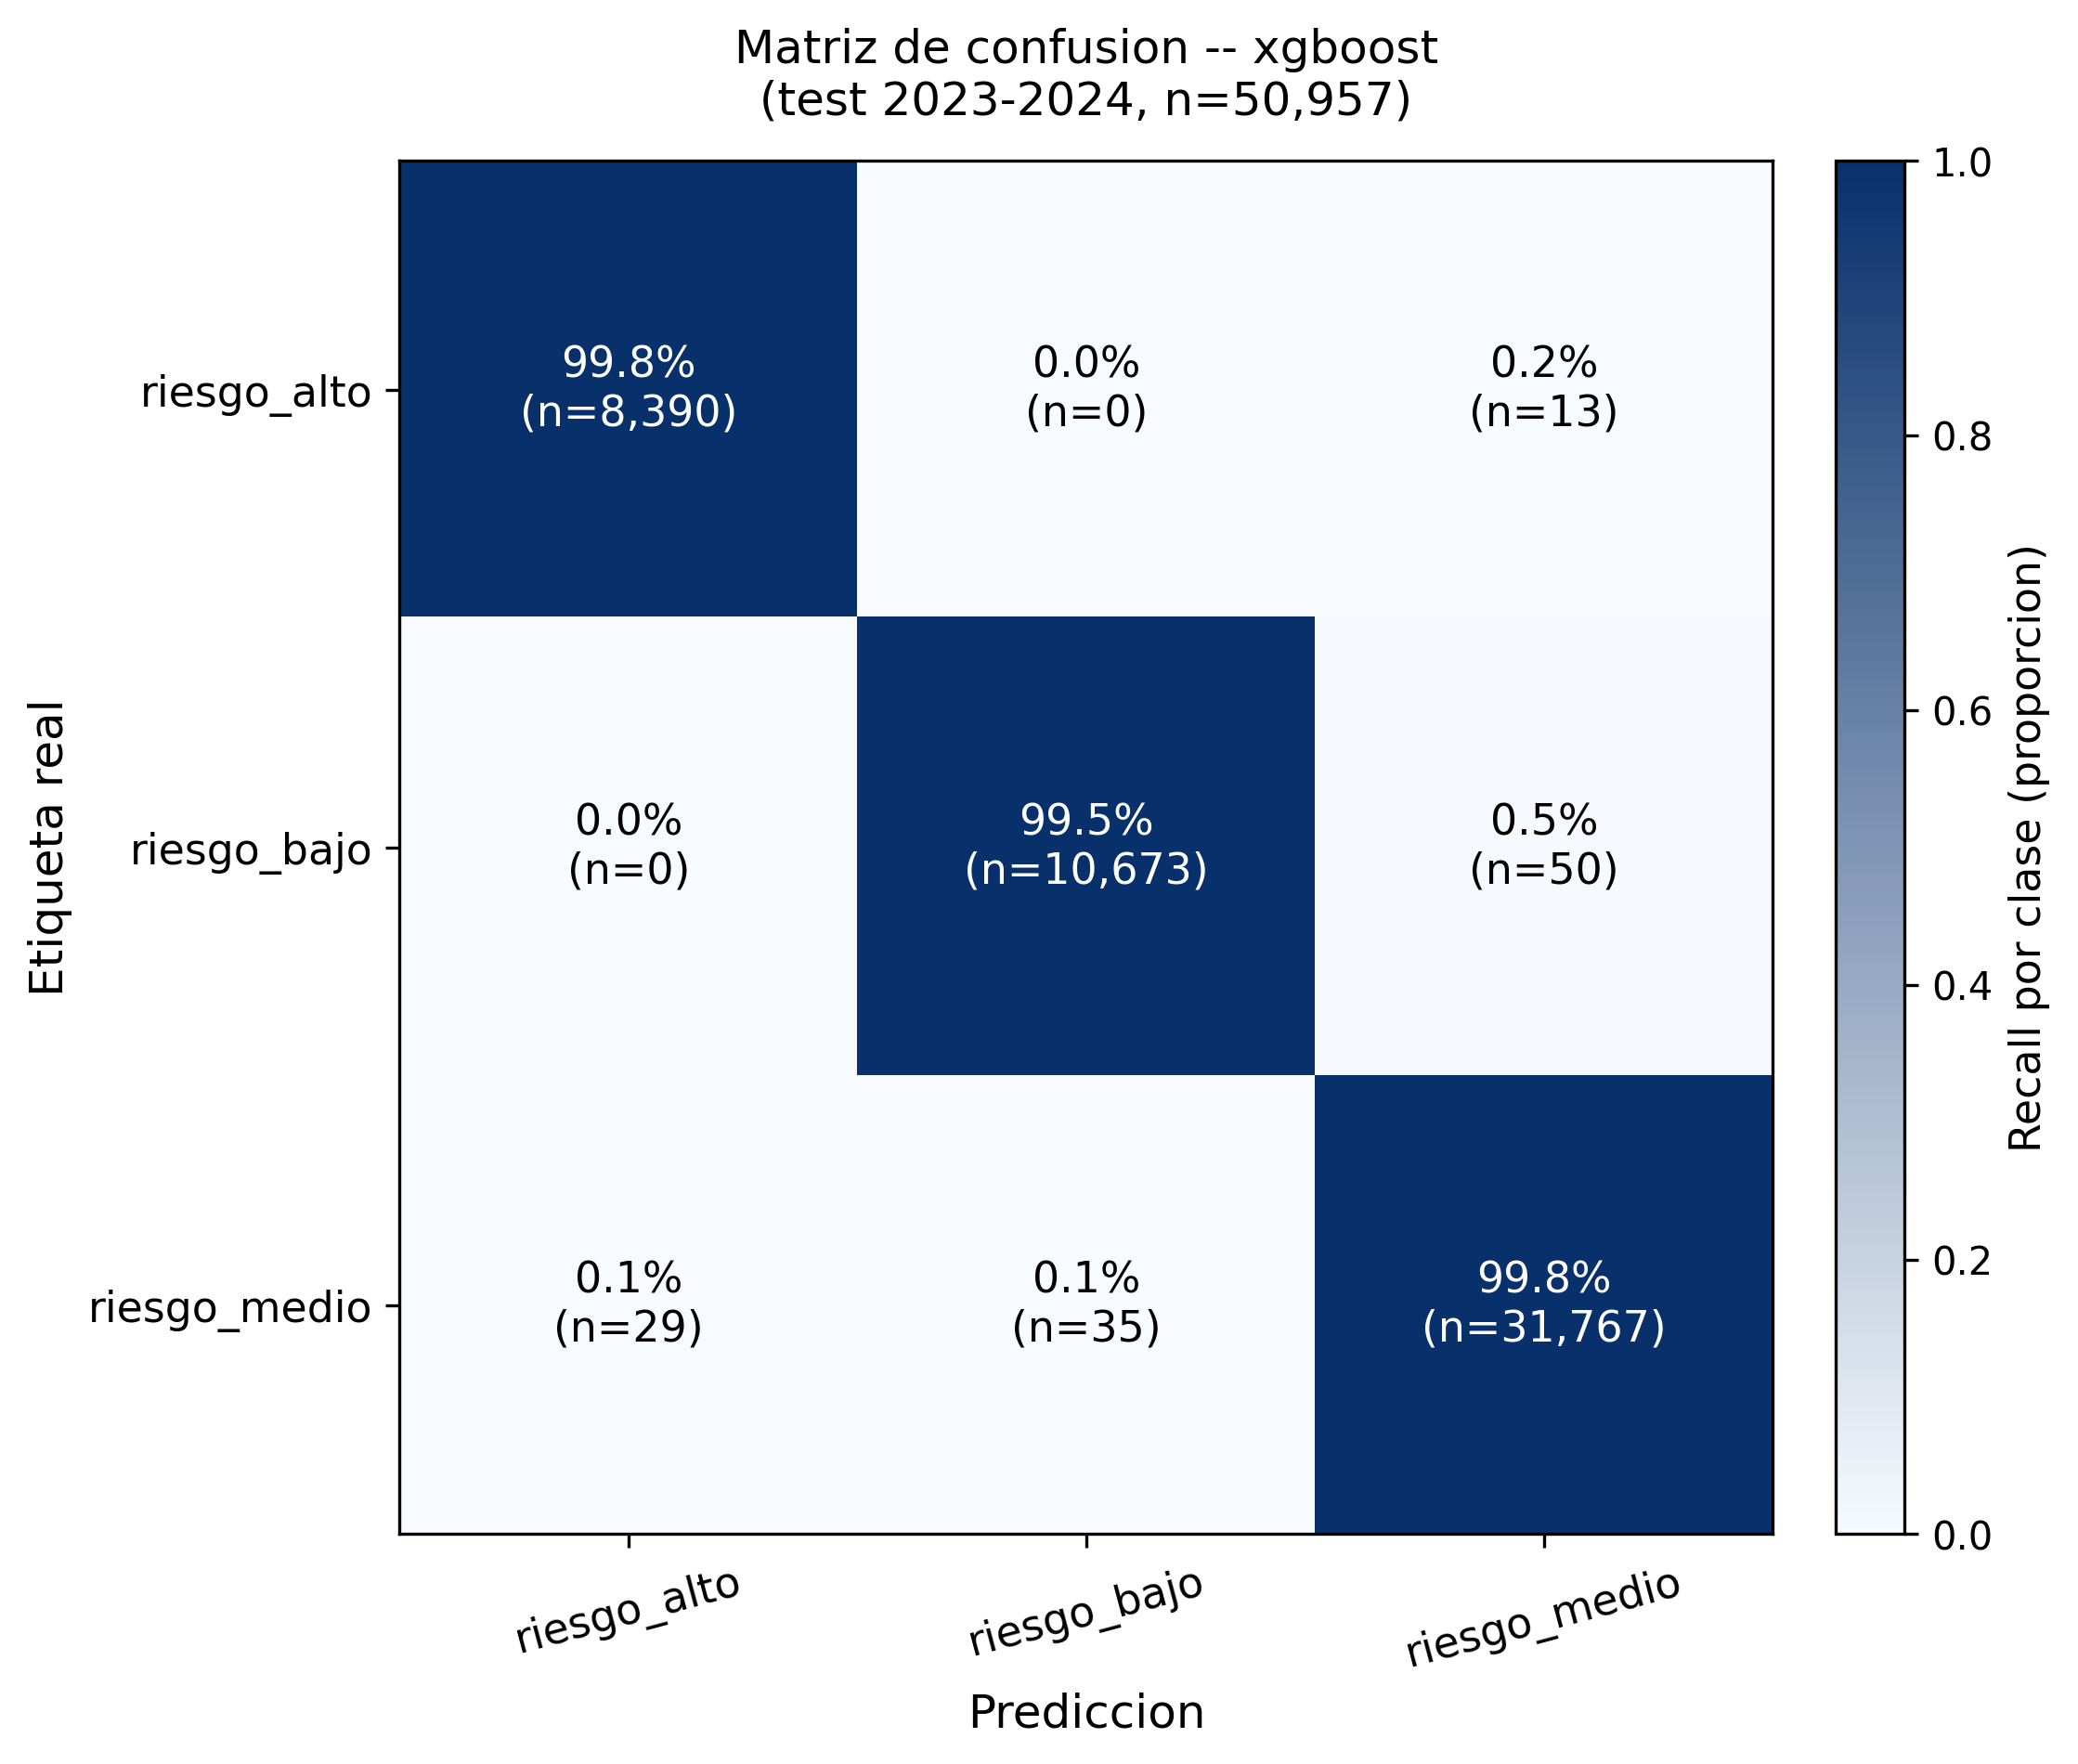
\includegraphics[height=5.2cm]{08_matriz_confusion_xgboost.png}
\smallskip
\begin{itemize}
  \item 127 errores en 50\,957 obs.\ (\textbf{0,25\%}). \emph{Recall} alto 99,85\%, bajo 99,53\%, medio 99,80\%.
  \item Errores concentrados en fronteras alto$\leftrightarrow$medio y bajo$\leftrightarrow$medio (zona gris natural).
\end{itemize}
\end{frame}

% =====================================================================
% Slide 14 - SHAP global
% =====================================================================
\begin{frame}{Interpretaci\'on TreeSHAP global}
\centering
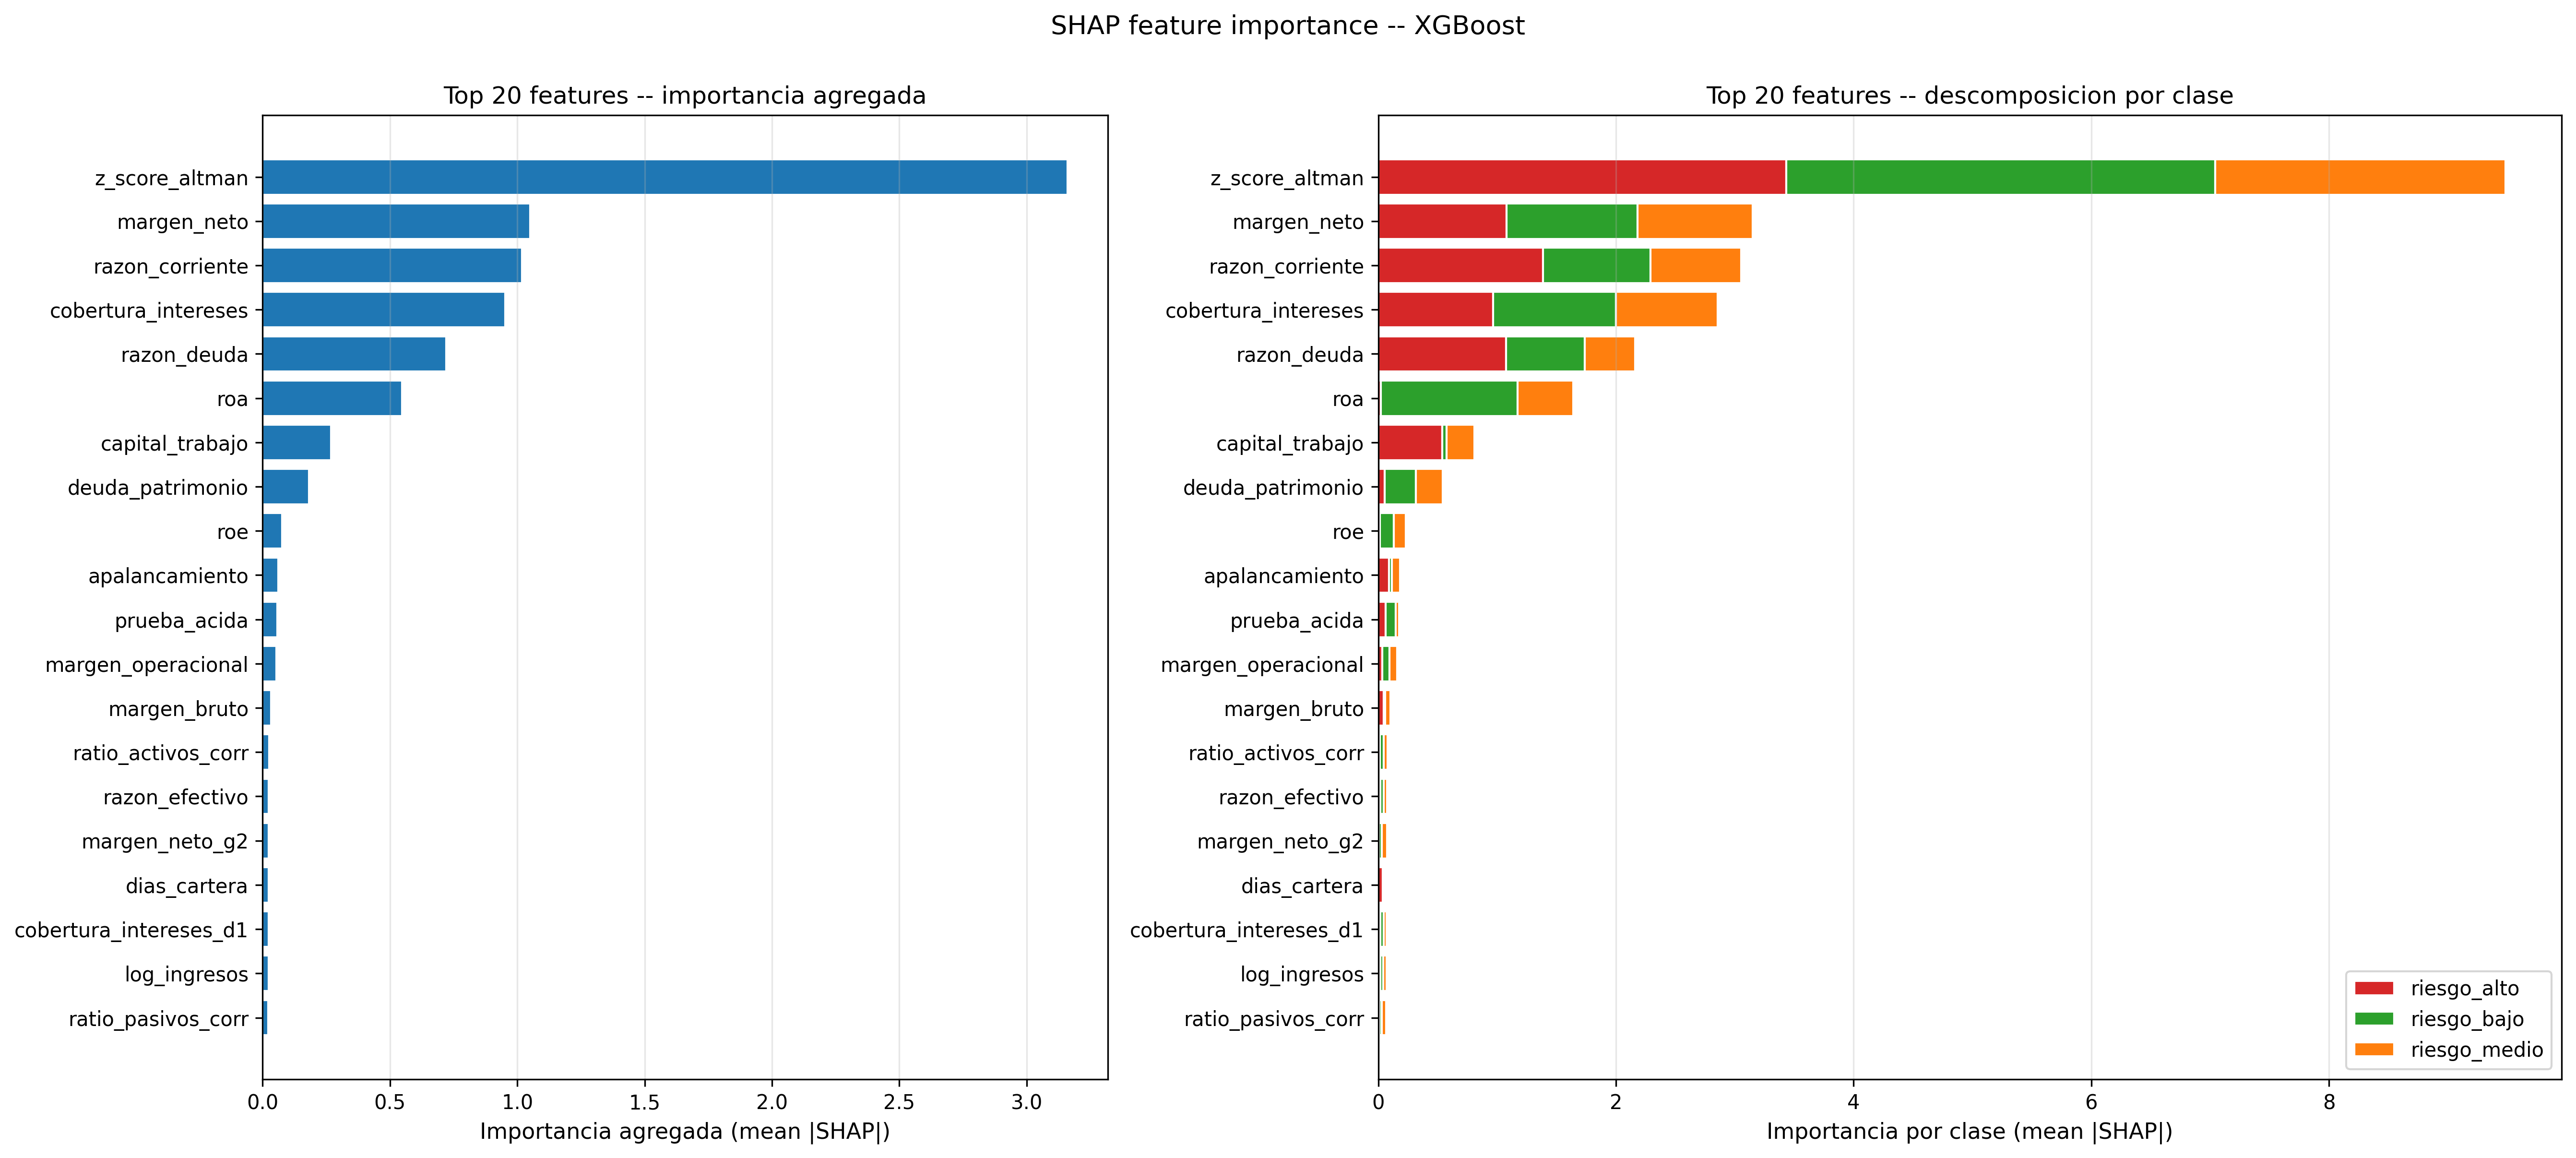
\includegraphics[height=4.6cm]{12_shap_importance_bar.png}
\smallskip
\begin{itemize}
  \item Top: \texttt{z\_score\_altman} (3,16) $>$ \texttt{margen\_neto} $>$ \texttt{razon\_corriente} $>$ \texttt{cobertura\_intereses}.
  \item 7/9 \emph{features} esperadas por la literatura aparecen en el top 10 [Bussmann 2020].
  \item Dominancia de \zaltscore{} ($\sim 3\times$ el segundo) refleja circularidad parcial del consenso B$\equiv$C.
\end{itemize}
\end{frame}

% =====================================================================
% Slide 15 - Validacion Ibague
% =====================================================================
\begin{frame}{Validaci\'on en Ibagu\'e (61 PYMES, 359 obs.)}
\begin{itemize}
  \item F1-macro Ibagu\'e \emph{sin} 2017 $= \mathbf{0{,}9948}$; gap vs.\ test nacional $= +0{,}24$ pp ($\leq 10$ pp $\checkmark$).
  \item AUC-ROC OvR $= 1{,}0000$; F1-macro 2016--2023 $= 1{,}0000$; 2024 $= 0{,}9640$.
  \item \textbf{Un solo error} en 359 predicciones --- NIT \texttt{*043005}, 2024:
  \begin{itemize}
    \item Real $=$ riesgo bajo, predicho $=$ riesgo medio (probabilidad 0{,}66).
    \item \zaltscore{} $= 6{,}95$ (sano), pero la \texttt{cobertura\_intereses} cay\'o 95\% YoY (de 34 a 1{,}66).
    \item El modelo capta esta volatilidad operativa que la heur\'istica nivel-base no observa.
  \end{itemize}
\end{itemize}
\end{frame}

% =====================================================================
% Slide 16 - vs Metodos clasicos
% =====================================================================
\begin{frame}{Discusi\'on: vs.\ m\'etodos cl\'asicos}
\centering
\small
\setlength{\tabcolsep}{6pt}
\renewcommand{\arraystretch}{1.1}
\begin{tabular}{@{}l c c@{}}
\toprule
\textbf{M\'etodo} & \textbf{F1-macro test} & \textbf{$\Delta$ vs.\ XGBoost} \\
\midrule
\textbf{XGBoost}                   & \textbf{0,9972} & --- \\
Random Forest                      & 0,9943 & $-0{,}3$ pp \\
Regresi\'on log\'istica            & 0,8105 & $-18{,}7$ pp \\
Altman terciles emp\'iricos        & 0,6891 & $\mathbf{-30{,}8}$ pp \\
Altman umbrales originales         & 0,4371 & $\mathbf{-56{,}0}$ pp \\
\bottomrule
\end{tabular}
\medskip
\begin{itemize}
  \item \textbf{$+30{,}8$ pp sobre Altman terciles} cuantifica la contribuci\'on marginal del ML.
  \item Heur\'istica EE.UU.\ degrada en PYMES Colombia, en l\'inea con Grice 2003 / Bouwmeester 2020.
\end{itemize}
\end{frame}

% =====================================================================
% Slide 17 - vs Literatura + Robustez
% =====================================================================
\begin{frame}{Vs.\ literatura y pruebas de robustez}
\textbf{Comparaci\'on con la literatura:}
\begin{itemize}
  \item Boumhidi 2025 / Mahesh 2025 / Yufenyuy 2024 / Dasilas 2024: AUC $\approx 0{,}93$, Acc $\approx 93\%$, F1 $\approx 0{,}89$.
  \item \textbf{Este trabajo:} F1-macro $= 0{,}997$, AUC $\approx 1{,}0$ --- rango superior reportado.
\end{itemize}
\textbf{Robustez del modelo XGBoost:}
\begin{itemize}
  \item Temporal: F1 2023 $= 0{,}9970$ vs.\ 2024 $= 0{,}9973$ (gap 0,03 pp).
  \item Sectorial (top 5 CIIU): F1 entre 0,9958 y 0,9980 (gap 0,22 pp).
  \item SHAP 5 \emph{seeds}: top-3 estable al \textbf{100\%}, Jaccard top-10 $= 0{,}927$.
\end{itemize}
\end{frame}

% =====================================================================
% Slide 18 - Conclusiones
% =====================================================================
\begin{frame}{Conclusiones --- mapeo de objetivos}
\begin{itemize}
  \item \textbf{O1.} 18 indicadores + \zaltscore{} sobre 203\,104 obs (completitud 54,8--95,2\%). $\checkmark$
  \item \textbf{O2.} Etiqueta triangulada con $\kappa_{B,C}=0{,}446$ ($\geq 0{,}4$). $\checkmark$
  \item \textbf{O3.} Cuatro modelos comparados; XGBoost gana val y test. $\checkmark$
  \item \textbf{O4.} F1-macro test $= 0{,}9972$, AUC-ROC OvR $= 0{,}99999$, sin \emph{drift}. $\checkmark$
  \item \textbf{O5.} TreeSHAP: 7/9 \emph{features} de literatura en top 10; 9 \emph{waterfalls} locales. $\checkmark$
  \item \textbf{O6.} F1 Ibagu\'e $= 0{,}9948$, gap $+0{,}24$ pp vs.\ nacional, 1 error en 359. $\checkmark$
\end{itemize}
\end{frame}

% =====================================================================
% Slide 19 - Limitaciones y trabajo futuro
% =====================================================================
\begin{frame}{Aportes, limitaciones y trabajo futuro}
\textbf{Aportes principales}
\begin{itemize}
  \item Primer ML interpretable sobre 38\,245 PYMES colombianas bajo NIIF.
  \item Contribuci\'on marginal cuantificada: $+56$ pp vs.\ Altman puro.
  \item \emph{Pipeline} reproducible (notebooks 03--10) --- base directa para una eventual interfaz web.
\end{itemize}
\textbf{Limitaciones / trabajo futuro}
\begin{itemize}
  \item Sesgo SIREM, etiqueta como \emph{proxy}, anomal\'ia 2017, dominancia del \zaltscore{} en SHAP.
  \item Integraci\'on web; fuentes complementarias (Confec\'amaras, DIAN); horizontes 1/2/3 a\~nos; validaci\'on contra eventos reales de liquidaci\'on.
\end{itemize}
\end{frame}

% =====================================================================
% Slide 20 - Cierre / Preguntas
% =====================================================================
{\setbeamercolor{background canvas}{bg=uibblue}
\setbeamercolor{normal text}{fg=white}
\begin{frame}[plain]
\centering
\vspace{1.3cm}
{\color{white}\Huge\bfseries \textquestiondown Preguntas?\par}
\vspace{1.3cm}
{\color{white}\Large Gracias por su atenci\'on\par}
\vspace{1.0cm}
{\color{white}\normalsize Juan Camilo Perea \quad\textbar\quad German\par}
{\color{white!85!uibblue}\small Universidad de Ibagu\'e --- 2026\par}
\end{frame}}

\end{document}
